\documentclass[11pt,a4paper]{article}
\usepackage{iftex}
\ifPDFTeX
  \usepackage[T1]{fontenc}
  \usepackage[utf8]{inputenc}
\else
  \usepackage{fontspec}
\fi
\usepackage[spanish,es-noshorthands]{babel}
\usepackage{amsmath,amssymb}
\usepackage{booktabs}
\usepackage{graphicx}
\usepackage{geometry}
\usepackage{float}
\usepackage{hyperref}
\geometry{margin=2.3cm}
\graphicspath{{../results/tabla/graficas/}}
\hypersetup{colorlinks=true,linkcolor=black,urlcolor=blue}
\title{Tabla I hasta $N=8640$\\[0.3em]
\large Contraste con Fasolino, Los y Katsnelson (2007)}
\author{Emanuel Orozco Gallego}
\date{11 de noviembre de 2026}
\begin{document}
\maketitle
\begin{abstract}
Se reimplementa el Monte Carlo del paper para todos los tamaños de la Tabla~I con $N\le 8640$: 240, 960, 2160, 4860 y 8640, a $T=300\,\mathrm{K}$. $N=19940$ queda fuera del tope. $T=3500\,\mathrm{K}$ (Figs.~4 y~5) no se simula. El potencial es Tersoff de Lindsay--Broido; el del paper es LCBOPII.
\end{abstract}

\section{Qué exige el paper}
Hoja plana, condiciones periódicas, $4\times 10^5$ pasos de equilibrado y $5\times 10^5$ de promediado. Un paso son $N$ intentos. Cada cinco pasos, una fluctuación isotrópica de área. Los observables son $h$, $G(q)=q^2|h_q|^2$ y $g(r)$. La referencia armónica es $G_0(q)/N=T/(\kappa S_0 q^2)$ con $\kappa=1.1\,\mathrm{eV}$. La Fig.~3 muestra que las dos cajas más cortas que $\sim 70\,\text{\AA}$ no tienen la caída de $G(q)$ a bajo $q$, y que las más largas sí, con un máximo cerca de $q\approx 0.1\,\text{\AA}^{-1}$. Para $N=8640$ citan una altura típica de orden $0.6\,\text{\AA}$. El primer pico de $g(r)$ a $300\,\mathrm{K}$ está en el enlace conjugado $1.42\,\text{\AA}$.

\section{Geometría}
La caja usada es $L_x=p|a_1|$ y $L_y=q\cdot 3a$, con $a=1.42\,\text{\AA}$ y $N=4pq$. Coincide con los números de la Tabla~I salvo el $L_x$ impreso de $N=960$ ($49.29\,\text{\AA}$): $p|a_1|=49.19\,\text{\AA}$. El resto de esa columna, y todas las demás filas, cierran con esta fórmula, así que se simula $49.19$ y no el valor impreso.

\begin{center}
\begin{tabular}{rrrrrrr}
\toprule
$N$ & $p$ & $q$ & $L_x$ & $L_y$ & Tabla $L_x$ & Tabla $L_y$ \\
\midrule
240 & 10 & 6 & 24.60 & 25.56 & 24.59 & 25.56 \\
960 & 20 & 12 & 49.19 & 51.12 & 49.29 & 51.12 \\
2160 & 30 & 18 & 73.79 & 76.68 & 73.78 & 76.68 \\
4860 & 45 & 27 & 110.68 & 115.02 & 110.68 & 115.02 \\
8640 & 60 & 36 & 147.57 & 153.36 & 147.57 & 153.36 \\
\bottomrule
\end{tabular}
\end{center}

\section{Resultados a $300\,\mathrm{K}$}
\begin{center}
\small
\begin{tabular}{rrrrrrr}
\toprule
$N$ & $h_{\mathrm{rms}}$ (\AA) & $E/N$ (eV) & acc.\ (\%) & pico $g(r)$ & $G/G_0$ & $q_{\min}$ \\
\midrule
240 & 0.180$\pm$0.007 & -7.939 & 39.2 & 1.435 & 0.73 & 0.243 \\
960 & 0.318$\pm$0.021 & -7.939 & 39.2 & 1.435 & 0.74 & 0.121 \\
2160 & 0.385$\pm$0.016 & -7.938 & 39.2 & 1.435 & 0.74 & 0.081 \\
4860 & 0.473$\pm$0.025 & -7.939 & 39.2 & 1.445 & 0.75 & 0.054 \\
8640 & 0.470$\pm$0.075 & -7.939 & 39.2 & 1.445 & 0.75 & 0.040 \\
\bottomrule
\end{tabular}
\end{center}

$G/G_0$ es la mediana en $q\in[0.40,1.20]\,\text{\AA}^{-1}$, lejos de $q_{\min}$ y del primer Bragg. Un valor de orden 1 dice que la convención de Fourier y $\kappa=1.1\,\mathrm{eV}$ describen esa ventana. $E/N$ se compara con la hoja plana de Tersoff, $-7.966\,\mathrm{eV}$. El pico de $g(r)$ se lee entre $1.2$ y $1.65\,\text{\AA}$ y se compara con $1.42\,\text{\AA}$.

Los ejes de las figuras siguientes se midieron sobre las Figs.~1, 3 y~5 del PDF en \texttt{references/}. La Fig.~3 es log--log con $q$ de $0.05$ a $5\,\text{\AA}^{-1}$ (dos décadas) y $G(q)/N$ de $10^{-3}$ a $1$ (tres décadas); el marco es más alto que ancho, en la proporción $202/156$ del original. La Fig.~4 usa ese mismo marco y añade la curva a $3500\,\mathrm{K}$, que aquí no está. La Fig.~5 usa $r$ de $0$ a $3.5\,\text{\AA}$ y un eje vertical de $0$ a $3$ etiquetado rdf.

\begin{figure}[H]
\centering
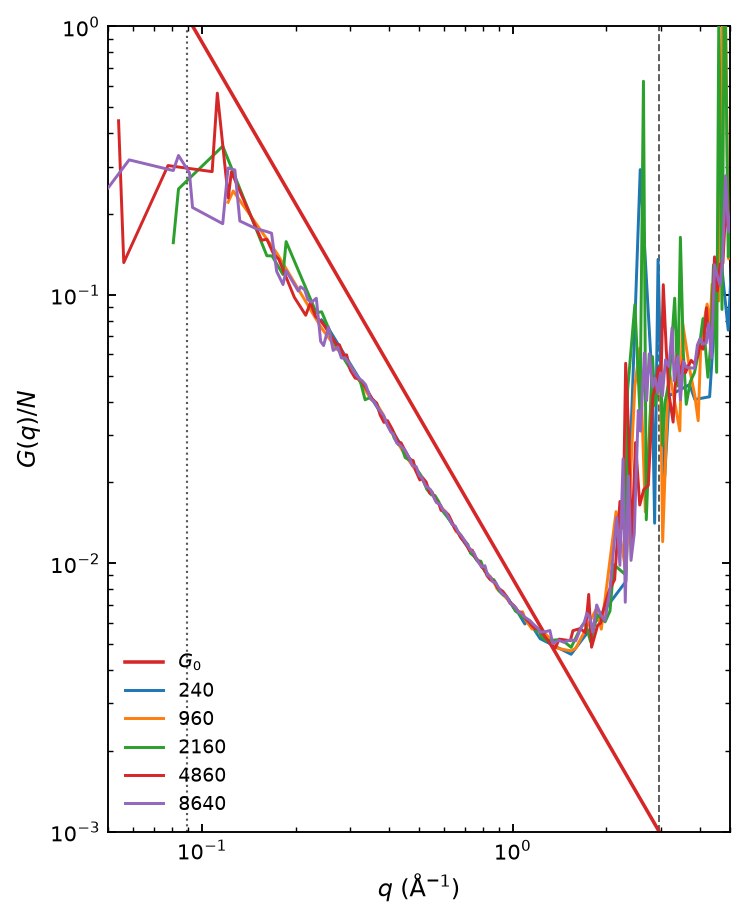
\includegraphics[width=0.62\textwidth]{Gq_fig3.png}
\caption{$G(q)/N$ en los ejes de la Fig.~3. La recta roja es $G_0$ con $\kappa=1.1\,\mathrm{eV}$. La punteada es $q=2\pi/70\,\text{\AA}$ y la discontinua el primer Bragg $4\pi/(3a)=2.94\,\text{\AA}^{-1}$. El segundo, $4\pi/(\sqrt{3}a)=5.11$, cae justo a la derecha de $q=5$, el borde del paper. $N=19940$ está en esa figura y no se simula.}
\end{figure}

\begin{figure}[H]
\centering
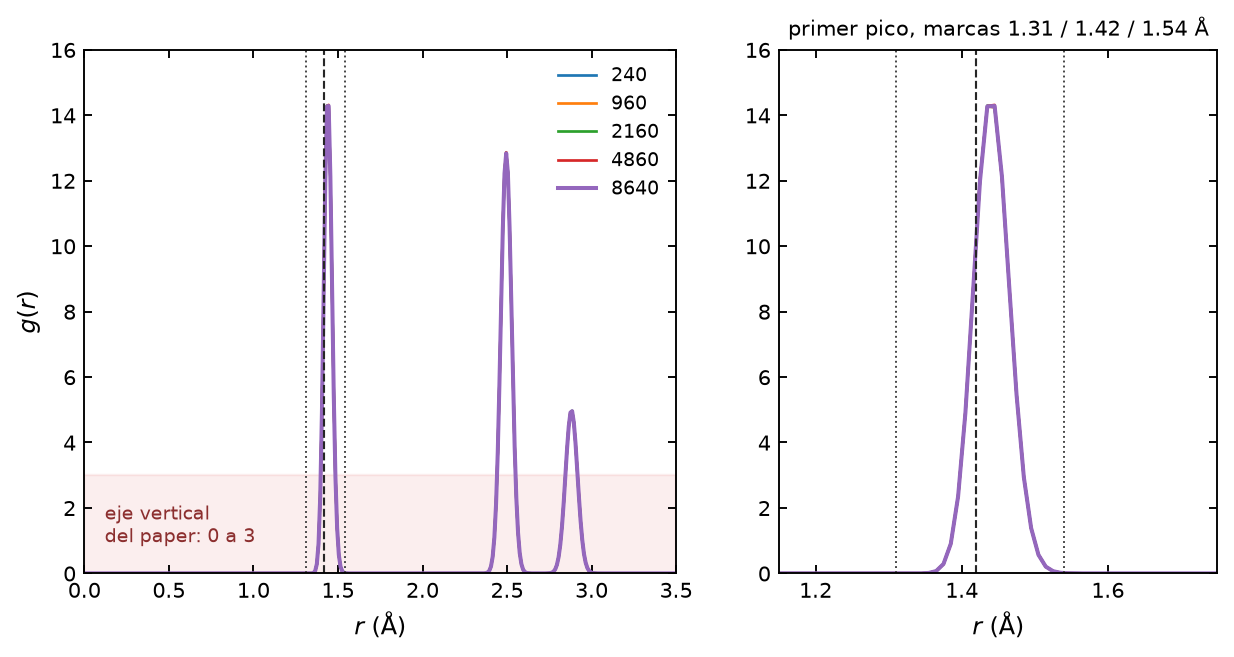
\includegraphics[width=0.92\textwidth]{rdf_fig5.png}
\caption{$g(r)$ con el eje horizontal de la Fig.~5 ($0$ a $3.5\,\text{\AA}$). Las marcas son el doble $1.31$, el conjugado $1.42$ y el simple $1.54\,\text{\AA}$. La banda roja es el eje vertical del paper, de $0$ a $3$. Aquí el bin es $0.01\,\text{\AA}$ y el primer pico llega a $\sim 14$: la altura no es la de esa figura; la posición sí. El panel derecho abre el primer pico. No hay hombros en $1.31$ ni en $1.54\,\text{\AA}$: haría falta la corrida a $3500\,\mathrm{K}$ con LCBOPII.}
\end{figure}

\begin{figure}[H]
\centering
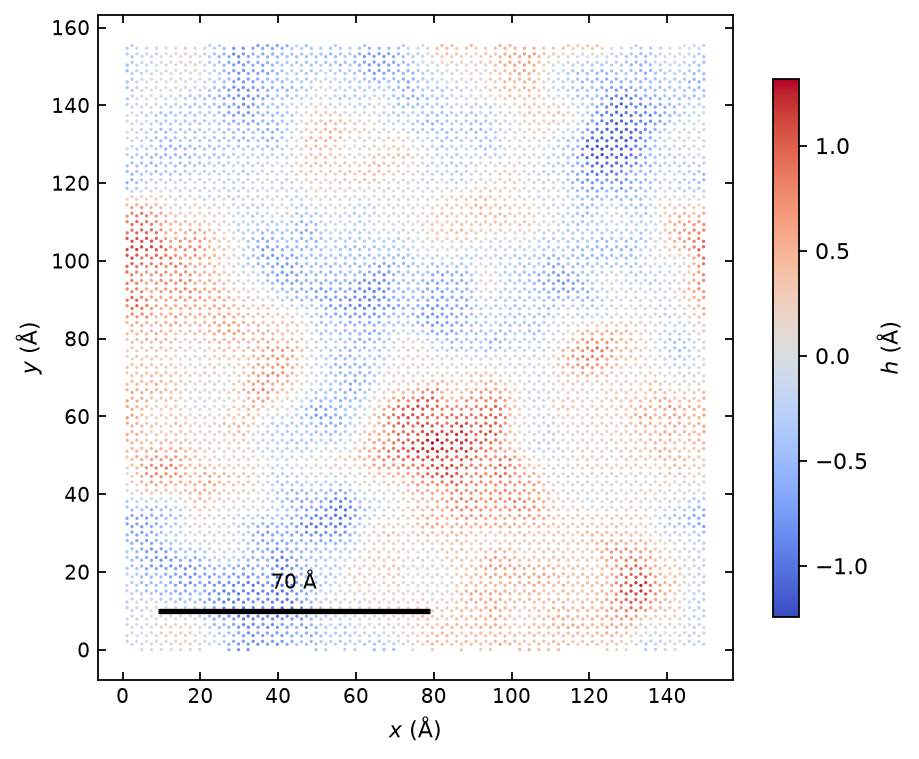
\includegraphics[width=0.72\textwidth]{snapshot_fig1.png}
\caption{Vista de la hoja $N=8640$ a $300\,\mathrm{K}$, con la barra de $70\,\text{\AA}$ que el paper dibuja sobre la Fig.~1. El color es la altura $h$ respecto del centro de masa. La altura típica que citan es $\sim 0.6\,\text{\AA}$; $h_{\mathrm{rms}}$ de esta corrida es $0.47\,\text{\AA}$.}
\end{figure}

\begin{figure}[H]
\centering
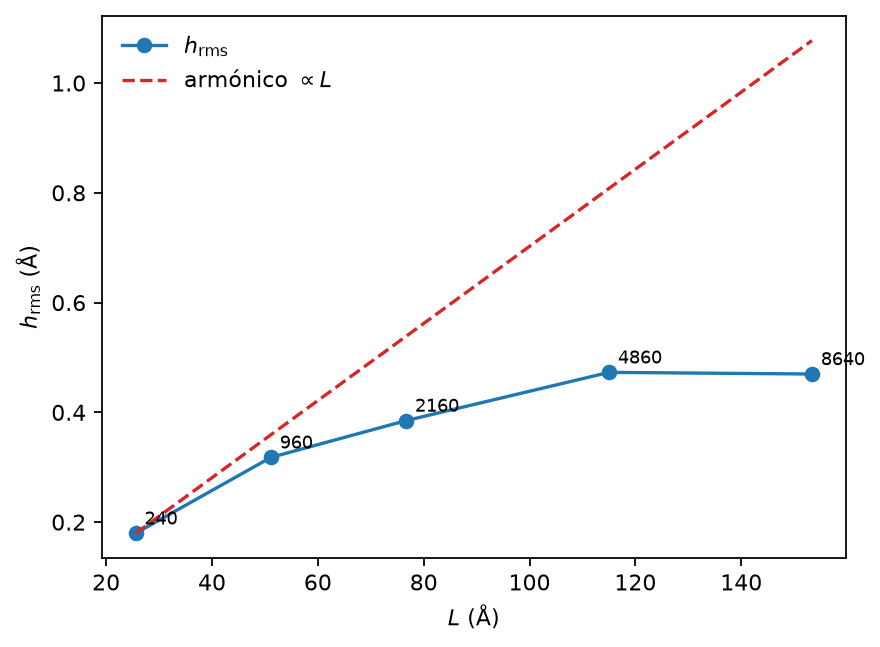
\includegraphics[width=0.72\textwidth]{hrms_vs_L.png}
\caption{$h_{\mathrm{rms}}$ frente al lado largo. Esta curva no está en el paper. La recta roja es el crecimiento armónico $\propto L$ anclado en $N=240$. Quedar por debajo es la supresión anarmónica que discuten a partir de la ec.~(4).}
\end{figure}

\section{Tamaño por tamaño}
\paragraph{$N=240$.} El paper dice que esta caja, más corta que 70~\AA, no muestra la caída de $G(q)$ a bajo $q$. El modo $q\approx 0.1$~\AA$^{-1}$ no cabe ($q_{\min}=0.243$).

\paragraph{$N=960$.} El paper dice que esta caja, más corta que 70~\AA, no muestra la caída de $G(q)$ a bajo $q$. El modo $q\approx 0.1$~\AA$^{-1}$ no cabe ($q_{\min}=0.121$).

\paragraph{$N=2160$.} Por debajo de $q\sim 0.1$~\AA$^{-1}$, $G(q)$ deja de seguir a $G_0\propto 1/q^2$ y el primer cascarón queda por debajo del máximo de la ventana $0.08$--$0.16$. Ese máximo es ancho y, con dos o cuatro réplicas, la dispersión es del orden de la bajada: no es el pico agudo de $\sim 70$~\AA\ que el paper asigna a la conjugación de LCBOPII. Tersoff no tiene ese canal.

\paragraph{$N=4860$.} Por debajo de $q\sim 0.1$~\AA$^{-1}$, $G(q)$ deja de seguir a $G_0\propto 1/q^2$ y el primer cascarón queda por debajo del máximo de la ventana $0.08$--$0.16$. Ese máximo es ancho y, con dos o cuatro réplicas, la dispersión es del orden de la bajada: no es el pico agudo de $\sim 70$~\AA\ que el paper asigna a la conjugación de LCBOPII. Tersoff no tiene ese canal.

\paragraph{$N=8640$.} Por debajo de $q\sim 0.1$~\AA$^{-1}$, $G(q)$ deja de seguir a $G_0\propto 1/q^2$ y el primer cascarón queda por debajo del máximo de la ventana $0.08$--$0.16$. Ese máximo es ancho y, con dos o cuatro réplicas, la dispersión es del orden de la bajada: no es el pico agudo de $\sim 70$~\AA\ que el paper asigna a la conjugación de LCBOPII. Tersoff no tiene ese canal.

\section{Qué no se reproduce}
\begin{itemize}
\item $N=19940$ ($p=90$, $q=54$): está en la Tabla~I y pasa de 8640.
\item $T=3500\,\mathrm{K}$: Figs.~4 y~5. El máximo se desplaza a unos $30\,\text{\AA}$ y $g(r)$ muestra hombros de enlace simple y doble. Hace falta LCBOPII.
\item El pico agudo de $70\,\text{\AA}$ es, en el paper, consecuencia del canal de conjugación de LCBOPII. Tersoff no tiene ese canal. La meseta ancha a bajo $q$ no se presenta como ese pico.
\end{itemize}
\end{document}
